\subsection*{A.1 Experiments, scripts and artefacts}
All code is in \texttt{code/}; \texttt{code/README.md} gives the commands. Each experiment is a function in \texttt{code/experiments.py}, run with \texttt{python sweep.py <name> <n\_procs>}, which appends one JSON line per run (including the full accuracy/loss/parameter-norm curve) to \texttt{results/<name>.jsonl}.
\texttt{python analysis.py} regenerates every figure (\texttt{paper/figs}), table (\texttt{paper/tables}) and number quoted in the text (\texttt{results/summary.json}).
\begin{center}\scriptsize
\begin{tabular}{p{2.3cm}p{5.8cm}p{1.1cm}p{3.2cm}}\toprule
Experiment & Configuration (seeds) & Runs & Used for\\\midrule
\texttt{e1\_mlp\_width} & MLP, $p{=}53$, add, $f{=}0.3$, $w\in\{24,\dots,512\}$ (10 widths), $T_{max}{=}10^5$ (100--105) & 60 & Fig.~\ref{fig:e1}, Tab.~\ref{tab:e1}, Fig.~\ref{fig:probe}c, \ref{fig:thresh}\\
\texttt{e2\_random} & as e1, random train labels (100--102) & 30 & Fig.~\ref{fig:probe}\\
\texttt{e3\_frac} & $f\in\{0.2,0.5\}$, $w\in\{24..256\}$, real (100--102) and random labels (100--102), $T_{max}{=}6\!\times\!10^4$ & 96 & Fig.~\ref{fig:probe}, \ref{fig:thresh}, \ref{fig:frac}\\
\texttt{e8\_small} & $w\in\{8,12,16,20\}$, $f\in\{0.2,0.3,0.5\}$, real and random labels (100--103), $T_{max}{=}6\!\times\!10^4$ (added after seeing that e2 fits from $w{=}24$) & 96 & Fig.~\ref{fig:probe}, \ref{fig:thresh}\\
\texttt{e10\_threshold} & $w\in\{72,80,88\}$, $f{=}0.3$ (100--105), $10^5$ steps (post hoc) & 18 & Sec.~\ref{sec:thresh}\\
\texttt{e9\_long} & $w\in\{48,64\}$, $f{=}0.3$, $T_{max}{=}4\!\times\!10^5$ (100--102) (post hoc) & 6 & Fig.~\ref{fig:thresh}\\
\texttt{e4\_timescale} & $w{=}128$; 7 (lr,wd) pairs; $T_{max}{=}8\!\times\!10^4$ (100--103) & 28 & Fig.~\ref{fig:e4}\\
\texttt{e11\_saturation} & $w{=}384$; (lr,wd)$\in\{(2\!\times\!10^{-3},1),(10^{-3},3)\}$; $T_{max}{=}6\!\times\!10^4$ (100--103) (post hoc, P8) & 8 & Sec.~\ref{sec:timescale}\\
\texttt{e6\_generality} & sub, mul, $a^2{+}b^2$ ($p{=}53$) and add ($p{=}97$), $w\in\{64,128,256\}$ (100--103; 100--102 for $p{=}97$) & 45 & Tab.~\ref{tab:e6}, Fig.~\ref{fig:e6}\\
\texttt{e7\_param} & lr$\propto1/w$, wd$\propto w$ or fixed; $w\in\{64..512\}$ (100--103; 100--101 at $w{=}512$) & 28 & Fig.~\ref{fig:e7}, Tab.~\ref{tab:e7}\\
\texttt{e5\_tf}, \texttt{e5b\_tf\_small}, \texttt{e12\_tf128\_long} & transformer, $d_{model}\in\{16,32,64,128\}$, $p{=}53$, $T_{max}{=}4\!\times\!10^4$ (100--103); $d_{model}{=}128$ re-run with $T_{max}{=}10^5$ (100--102, post hoc) & 16 + 3 & Sec.~\ref{sec:robust}, Fig.~\ref{fig:e5}, Tab.~\ref{tab:e5}\\
\texttt{pilot}, \texttt{pilot\_mlp} & exploratory pilot (seeds 0--2, 30k steps); both aborted when the compute budget was re-planned (partial) & 17 & motivates hypotheses only; not used in any reported statistic\\\bottomrule
\end{tabular}
\end{center}

\subsection*{A.2 Additional tables and figures}
\begin{table}[h]\centering\scriptsize
\caption{Width-scaling variants (Fig.~\ref{fig:e7}). The two scaled settings coincide at the reference width $w{=}128$ (same configuration and seeds).}\label{tab:e7}
\begin{tabular}{llrcccc}
\toprule
setting & width & lr & $t_{train}$ & $t_{val}$ & $R$ & cens./$n$ \\
\midrule
fixed lr, wd & 64 & 0.001 & 210 & $\geq$100000 [100000,100000] & $\geq$476 & 6/6 \\
fixed lr, wd & 128 & 0.001 & 90 & 37200 [26900,53200] & 413 & 0/6 \\
fixed lr, wd & 256 & 0.001 & 40 & 19700 [16500,20700] & 492 & 0/6 \\
fixed lr, wd & 512 & 0.001 & 20 & 16300 [13200,19500] & 815 & 0/6 \\
lr$\propto1/w$, lr$\cdot$wd fixed & 64 & 0.002 & 115 & $\geq$100000 [100000,100000] & $\geq$871 & 4/4 \\
lr$\propto1/w$, lr$\cdot$wd fixed & 128 & 0.001 & 90 & 37800 [21400,63200] & 420 & 0/4 \\
lr$\propto1/w$, lr$\cdot$wd fixed & 256 & 0.0005 & 60 & 24100 [21000,25800] & 402 & 0/4 \\
lr$\propto1/w$, lr$\cdot$wd fixed & 512 & 0.00025 & 45 & 18800 [18800,18800] & 423 & 0/2 \\
lr$\propto1/w$, wd fixed & 64 & 0.002 & 125 & $\geq$100000 [92800,100000] & $\geq$771 & 3/4 \\
lr$\propto1/w$, wd fixed & 128 & 0.001 & 90 & 37800 [21400,63200] & 420 & 0/4 \\
lr$\propto1/w$, wd fixed & 256 & 0.0005 & 60 & 46200 [34400,61600] & 770 & 0/4 \\
lr$\propto1/w$, wd fixed & 512 & 0.00025 & 45 & 76300 [65200,87400] & 1744 & 0/2 \\
\bottomrule
\end{tabular}
\end{table}
\begin{figure}[h]\centering
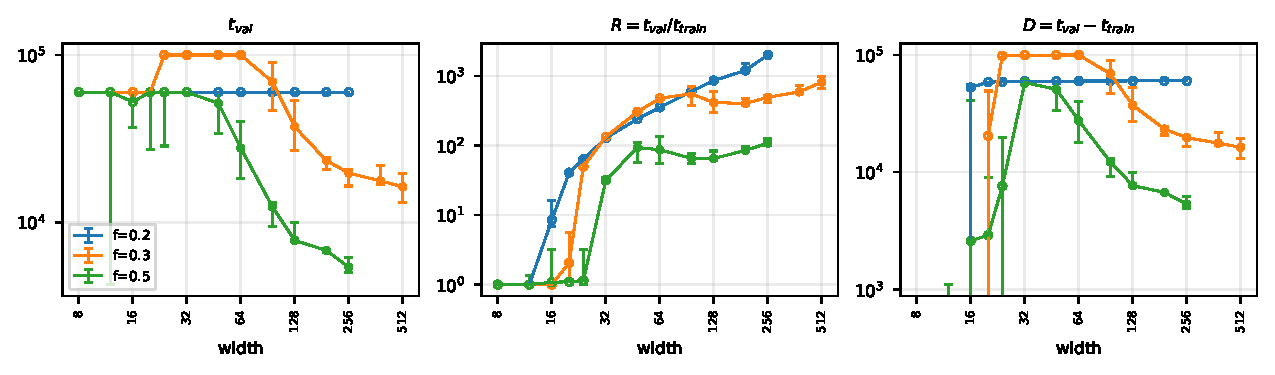
\includegraphics[width=.9\linewidth]{figs/fig_frac.pdf}
\caption{$t_{val}$, $R$, $D$ vs.\ width for three training fractions (MLP, $p{=}53$; $10^5$ steps for $f{=}0.3$, $6\!\times\!10^4$ for $f{=}0.2,0.5$; hollow: mostly censored). Only the $f{=}0.3$ line extends beyond $w{=}256$.}\label{fig:frac}
\end{figure}
\begin{figure}[h]\centering
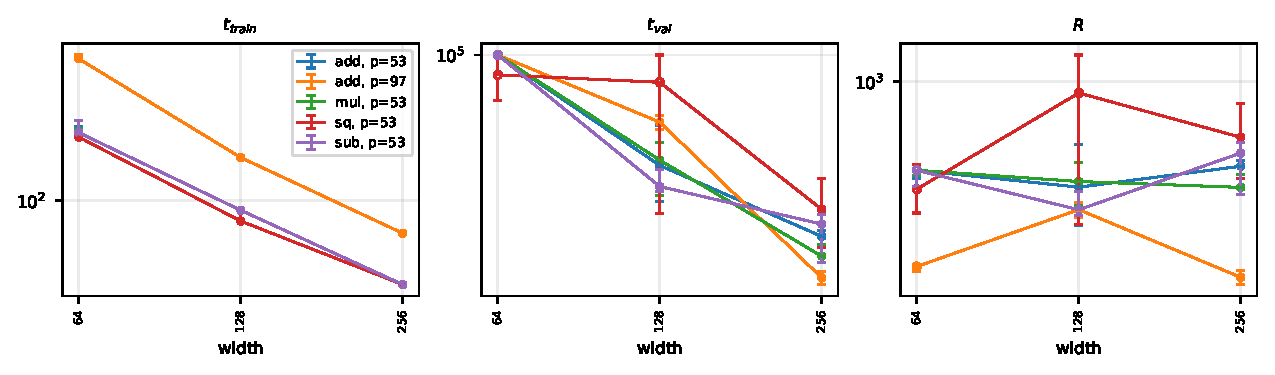
\includegraphics[width=.9\linewidth]{figs/fig_e6.pdf}
\caption{Other operations and modulus (Tab.~\ref{tab:e6}).}\label{fig:e6}
\end{figure}
\begin{table}[h]\centering\scriptsize
\caption{Transformer runs (seeds 100--103; 100--102 at $d_{model}{=}128$). Per-seed times to 99\% and (post hoc) 95\% validation accuracy; $-$: not reached within the budget. Max.\ val.\ acc.: highest validation accuracy over the run.}\label{tab:e5}
\begin{tabular}{rrrcccc}
\toprule
$d_{model}$ & params & budget & $t_{train}$ & $t_{val}$, 99\% (per seed) & $t_{val}$, 95\% (per seed) & max val.\ acc.\ \\
\midrule
16 & 5k & 40k & 1075 & $-$, $-$, $-$, $-$ & $-$, $-$, $-$, $-$ & 0.04, 0.02, 0.08, 0.04 \\
32 & 16k & 40k & 345 & $-$, $-$, $-$, $-$ & $-$, $-$, $-$, $-$ & 0.02, 0.07, 0.03, 0.02 \\
64 & 57k & 40k & 165 & $-$, 26.2k, 14.2k, 33.4k & $-$, 19.8k, 8.6k, 31.6k & 0.03, 0.99, 0.99, 0.99 \\
128 & 211k & 100k & 100 & $-$, 89.0k, $-$ & 27.4k, 88.0k, 14.4k & 0.99, 0.99, 0.99 \\
\bottomrule
\end{tabular}
\end{table}
\begin{figure}[h]\centering
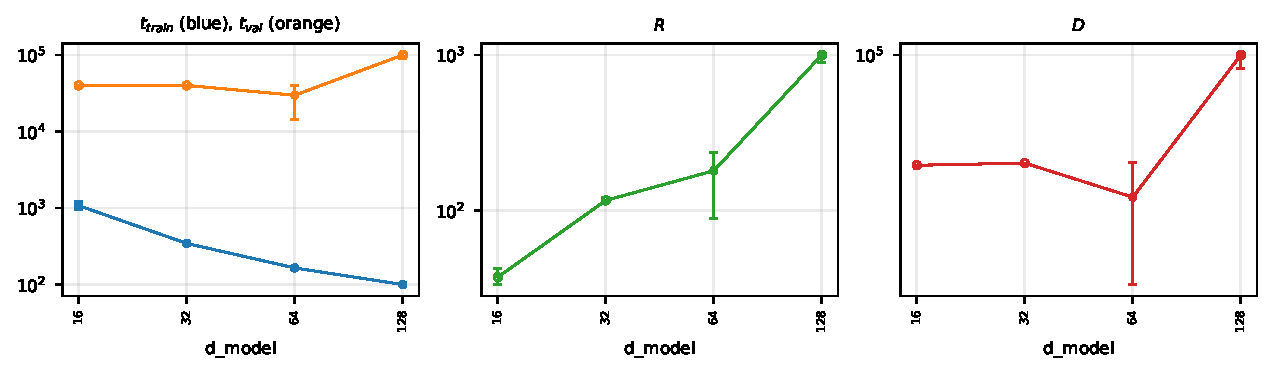
\includegraphics[width=.9\linewidth]{figs/fig_e5.pdf}
\caption{Transformer: $t_{train}$ and $t_{val}$ (99\%), $R$, $D$ vs $d_{model}$ (medians, bootstrap CIs; hollow: mostly censored).}\label{fig:e5}
\end{figure}

\subsection*{A.3 Environment, seeds, cost}
Python 3.11.15, PyTorch 2.15.0+cpu (CPU only, 1 thread per run), NumPy 2.4.6, SciPy 1.17.1, Matplotlib 3.11.2; LaTeX: TeX Live \texttt{pdflatex}/\texttt{latexmk}. Seeds: 0--2 (pilot), 100+ (all reported experiments); the seed sets both model initialisation and the train/validation split (split seed $=10000+$seed). Runs are deterministic for a given (config, seed) on a given machine (verified: duplicate configurations in e7 gave identical results).
The sandbox provided about 4--5 effective CPU cores shared with other tenants; the per-run wall-clock seconds in \texttt{results/*.jsonl} include contention. Summed per-run wall-clock time over all stored runs is given by \texttt{python code/compute\_stats.py} (\texttt{code/logs/compute\_stats.log}); it is 78 hours over all stored runs (434 reported runs plus 12 duplicated transformer runs and 17 pilot runs), most of it contention-inflated; the whole project took roughly 11 hours of wall-clock on this shared slice.

\subsection*{A.4 Deviations, failed or abandoned runs, and honest notes}
\begin{itemize}\setlength\itemsep{0pt}
\item \textbf{Template.} The official NeurIPS 2025 style file (the newest we could obtain: the 2026 archive was not available at the expected URL) is used in \texttt{preprint} mode (non-anonymous author line), with the NeurIPS checklist included.
\item \textbf{Compute-driven choices.} $p{=}53$ rather than $97$ (the latter is $\approx3\times$ costlier; checked only for 3 widths); transformer limited to $d_{model}\le128$ and $4\times10^4$ steps. An exploratory transformer pilot with $d_{model}$ up to 256 and an MLP pilot with $w\in\{512,1024\}$ were stopped for cost; their partial output is in \texttt{results/pilot*.jsonl} and is not used.
\item \textbf{Registration timing.} \texttt{PREREG.md} was written before e1 and e2 were launched. It is a self-registered file in the workspace (not an external registry), and the results of e2 (including the near-identical memorisation times) were visible before e3--e7 were launched; no prediction was changed afterwards, but P3's second half and the choice of e3/e4 grids could in principle have been influenced by e2.
\item \textbf{Post-hoc additions} (marked in the text): e8, e9, e10, e11, the three-regime interpretation, the saturation reading, and the choice to report $p{=}97$ for only 3 widths. The registered predictions P1--P7 were not edited after the sweeps (the file \texttt{code/PREREG.md} has an explicit addendum for P8).
\item \textbf{Analysis changes after seeing data.} The slope for $\ttr$ and $\tva$ is reported over fully-fitting/uncensored widths because including censored widths mixes bounds with values; the all-width slope for $\ttr$ is also given. The e4 regression treats censored runs as bounds (biased toward flatter slopes), a censoring-aware estimator (Tobit or survival regression) was not implemented. For the transformer, the 95\% validation criterion was added after observing plateaus just below 99\%.
\item \textbf{Parallel duplicates.} Because of a restart, some transformer configurations were queued twice; duplicate keys are dropped when loading (first result kept).
\item \textbf{Literature.} References were checked to exist via their arXiv abstract pages (\texttt{code/check\_refs.py}, \texttt{code/logs/refs\_check.log}); statements about their content in Sec.~2 follow the one-line descriptions in the task's starter list and our prior knowledge; the full texts were not re-read during this run. No other literature search was run.
\item \textbf{LLM usage.} The research design, code, experiments, analysis and this manuscript were produced by an autonomous LLM-based agent running unattended; no human reviewed the intermediate results. The studied models are small MLPs and transformers trained from scratch; no LLM is part of the experimental pipeline.
\item \textbf{Restricted content.} No search for, access to, or reading of the restricted paper(s) described in the task brief was performed; no web pages other than the NeurIPS style-file archive, pip packages and the arXiv abstract pages listed above were accessed. Nothing restricted was encountered.
\end{itemize}
